\documentclass[12pt]{article}
\usepackage{fullpage}

\usepackage[T1]{fontenc}
\usepackage[utf8]{inputenc}
\usepackage{lmodern}
\usepackage{microtype}
\usepackage[full]{textcomp}
\usepackage[osf]{newtxtext}
\usepackage{graphicx}

%% ---- Base math packages (always available) -------------------------------
\usepackage{amsmath, amssymb, amsthm, mathtools}
\usepackage{hyperref}

%% ---- Submission preamble (imported so the inlined solution compiles) ----
\usepackage{amsmath,amssymb,amsthm,mathtools}

\newtheorem{theorem}{Theorem}
\newtheorem{lemma}[theorem]{Lemma}
\newtheorem{proposition}[theorem]{Proposition}

\DeclareMathOperator{\Hilb}{Hilb}
\DeclareMathOperator{\grFrob}{grFrob}
\DeclareMathOperator{\Des}{Des}
\DeclareMathOperator{\des}{des}
\DeclareMathOperator{\maj}{maj}
\DeclareMathOperator{\shape}{shape}
\newcommand{\SYT}{\operatorname{SYT}}
\newcommand{\qbinom}[2]{\genfrac{[}{]}{0pt}{}{#1}{#2}_q}

%% ---- Theorem environments not supplied by the submission ------------------
\makeatletter
\@ifundefined{theorem}{\newtheorem{theorem}{Theorem}}{}
\@ifundefined{lemma}{\newtheorem{lemma}{Lemma}}{}
\@ifundefined{proposition}{\newtheorem{proposition}{Proposition}}{}
\@ifundefined{corollary}{\newtheorem{corollary}{Corollary}}{}
\@ifundefined{definition}{\theoremstyle{definition}\newtheorem{definition}{Definition}}{}
\@ifundefined{remark}{\theoremstyle{remark}\newtheorem{remark}{Remark}}{}
\makeatother

%% ---- First Proof theme + in-text comment box -----------------------------
%% Palette from the FINAL DELIVERABLES brand assets:
%%   slate     #171313  (ink)
%%   warm-gray #69626D  (secondary)
%%   sand      #F2ECE9  (light background)
\usepackage{xcolor}
\usepackage[most]{tcolorbox}

\definecolor{FPslate}{HTML}{171313}
\definecolor{FPwarmgray}{HTML}{69626D}
\definecolor{FPsand}{HTML}{F2ECE9}

% Reviewer number for this document (set per file). Used by the comment box tag.
\newcommand{\reviewernum}{2}

% \review{...} : a First-Proof-themed reviewer comment, set inline in the text
%            as a sand box with a warm-gray rule and a "Reviewer N" tag.
\newtcolorbox{reviewbox}{
  breakable, enhanced, sharp corners,
  colback=FPsand, colframe=FPwarmgray,
  coltext=FPslate, boxrule=0pt, leftrule=2.5pt,
  left=8pt, right=8pt, top=14pt, bottom=5pt,
  before skip=6pt, after skip=6pt,
  fontupper=\small,
  overlay unbroken and first={
    \node[anchor=north east, font=\bfseries\footnotesize\sffamily,
          text=FPwarmgray, inner sep=0pt]
      at ([xshift=-8pt,yshift=-4pt]frame.north east) {Reviewer~\reviewernum};}
}
\newcommand{\review}[1]{\begin{reviewbox}#1\end{reviewbox}}

\title{Review of Submission 9B}
\author{First Proof Second Batch \\ Reviewer \reviewernum}
\date{June 4--8, 2026}

\makeatletter
\renewcommand{\maketitle}{%
  \noindent
  \begin{minipage}[t]{0.68\textwidth}
    \vspace{20pt}
    \raggedright
    {\LARGE\bfseries \@title\par}
    \vspace{0.35em}
    {\large \@author\par}
    \vspace{0.35em}
    {\normalsize \@date\par}
  \end{minipage}%
  \hfill
  \begin{minipage}[t]{0.25\textwidth}
    \vspace{0pt}
    \raggedleft
    \raisebox{\dimexpr-\height+\ht\strutbox+0.225in\relax}{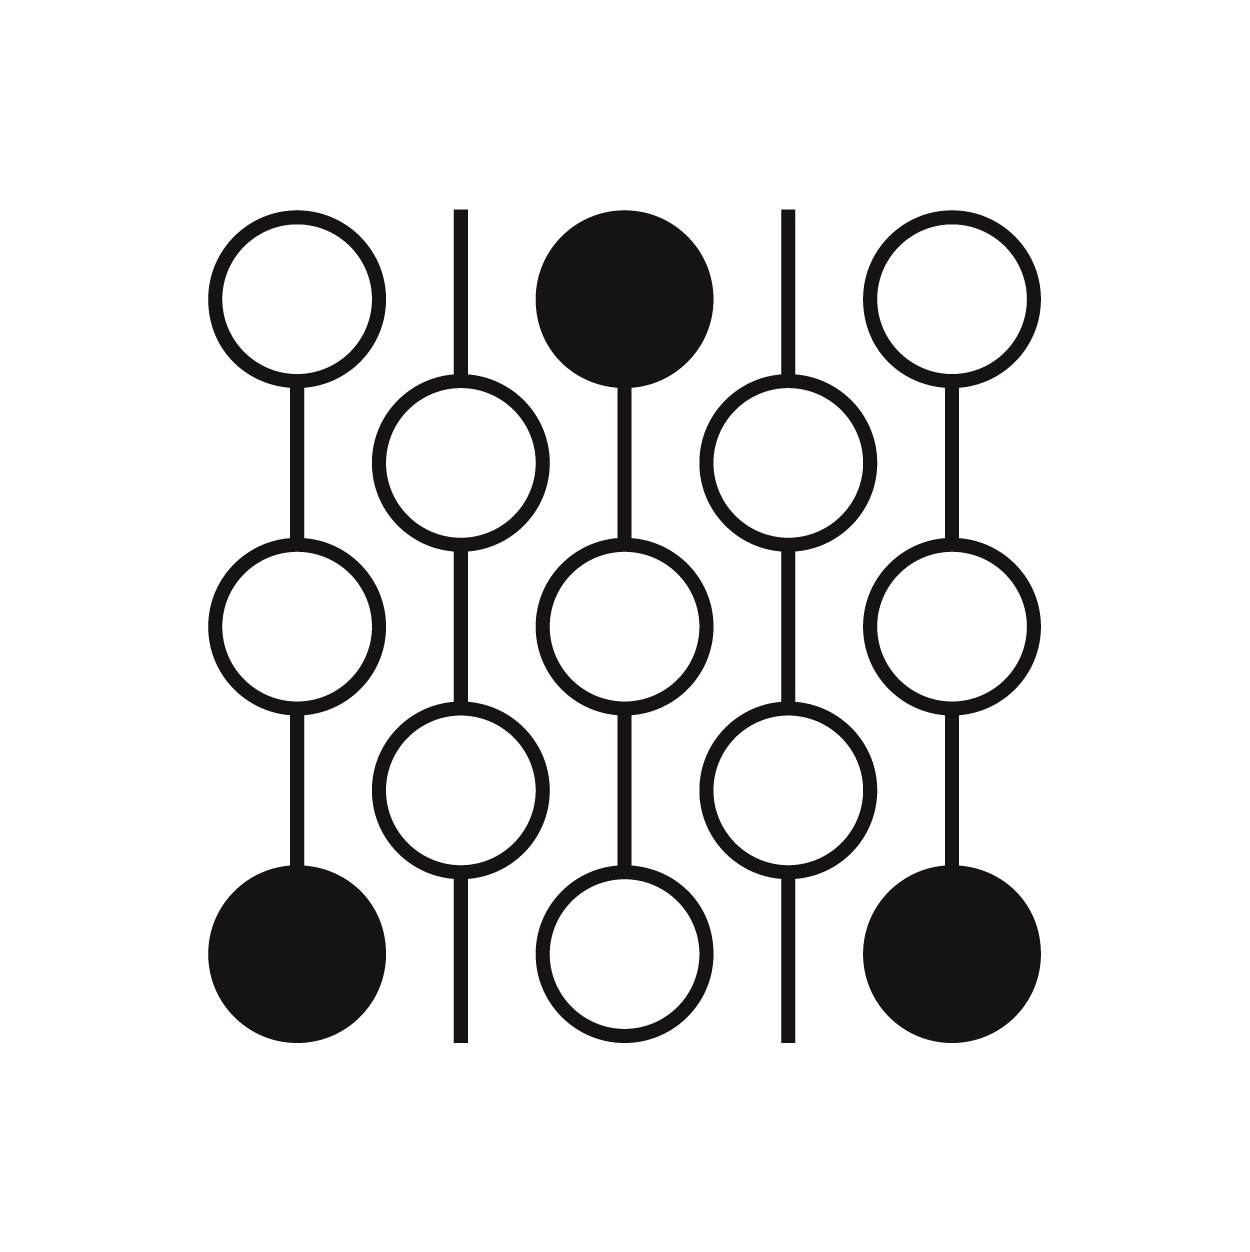
\includegraphics[height=1.35in]{Logo-slate.png}}
  \end{minipage}
  \par\vspace{2em}
}
\makeatother

\begin{document}
\maketitle
\section{Review}


\paragraph{Correctness.}
The submission appears to be entirely  correct, as far as I can tell.

\paragraph{Summary.}
This submission proves  the coefficients $\{c_{\lambda}(n): \lambda \text{ is a hook}\}$ count pairs $(w, \rho)$ of permutations $w$ and partitions $\rho$ satisfying several conditions depending on $\lambda$, $n$, and the descents of the permutation $w$. The main steps of the proof are:
\begin{enumerate}
    \item Using diagonal supersymmetry, show  that the Hilbert series for the \textit{superspace}\footnote{one-commuting, one-anticommuting variable} coinvariant ring can be written as sums of various $\{C_b\}$ where $C_b = \sum_{a \geq 1} c_{(a, 1^b)}(n)q^a$.
    \item Uses the Murai--Rhoades--Wilson Frobenius series for the superspace coinvariant ring to derive another formula for its Hilbert series.
    \item By comparing the formulations for the Hilbert series in (1) and (2), and using induction, it obtains another formula for $C_b$, involving permutations and descents. 
    \item Prove by $q$-identities that  that the proposed combinatorial interpretation matches the coefficient of $q^a$ in the formulation of $C_b$ in (3).
\end{enumerate}


\paragraph{Attributions.} Unlike the others, this submission does \textit{not} seem to plagiarize! On the other hand, it does seem to be unaware of key papers in the field (such as the Rhoades--Wilson Forum of Math. Pi. '24 paper). The knowledge of this paper would likely have simplified some of its arguments (like in \S 3.3). It also includes proofs of a couple of classical or routine lemmas (like $q$-Pascal identities), which it could instead cite references for.

\paragraph{Novelty.}

Although correct, the ``combinatorial interpretation'' in some ways feels a bit contrived. The objects which are claimed to be counted (pairs of a permutation and partition satisfying certain conditions) only arise as indexes in the sums after manipulating $q$-series, and are not really ``used'' in the proof at all.

On the other hand, this interpretation is quite different from the other four I've seen: the three other model solutions and the human solution. The other four all involve ordered set partitions, whereas this one does not --   likely because it seemed unaware of the Rhoades--Wilson paper. This opens the (potentially easy, but maybe interesting) question for finding a bijection between the objects in this combinatorial interpretation and any of the others.

\paragraph{Exposition.}
The writing style is clear and easy-to-follow. It could easily be shortened if necessary (it reproves some classical formulas and overexplains some points), but I still found it the easiest to read.

\section{Recommendation}

I would categorize this solutions as publishable with minor revisions.


  \section{Submission with inline comments}

%% ======================================================================
%% Inlined verbatim from the anonymised submission prob_009-B.
%% ======================================================================
%
\date{}


\subsection*{Overview / Strategy}

The proof passes from the ordinary diagonal coinvariant algebra with \(m\) bosonic alphabets to the one-bosonic-one-fermionic coinvariant algebra \(SR_n\).  A diagonal supersymmetry theorem says that the same universal Schur coefficients \(c_\lambda(n)\) occur after replacing \(s_\lambda(q_1,\ldots,q_m)\) by the super Schur function \(s_\lambda(q/u)\).  In one bosonic and one fermionic variable, every nonempty non-hook shape vanishes, while
\[
s_{(a,1^b)}(q/u)=q^a u^b+q^{a-1}u^{b+1}.
\]
This gives a triangular relation between the hook generating functions \(C_b(q)=\sum_{a\ge 1}c_{(a,1^b)}(n)q^a\) and the coefficients \(D_b(q)=[u^b]\Hilb(SR_n;q,u)\).

The second input is the Fields Frobenius formula, proved by Murai--Rhoades--Wilson.  After forgetting the \(S_n\)-module structure and using the Robinson--Schensted descent correspondence, this formula becomes a sum over permutations \(w\in S_n\).  Extracting the coefficient of \(u^b\) introduces a Gaussian binomial coefficient.  The triangular relation is then solved by induction using the \(q\)-Pascal identity, and the Gaussian binomial is finally expanded as a generating function for partitions in a rectangle.  This yields the stated counting formula for hook coefficients.

\subsection{Definitions and headline theorem}

For \(m,n\ge 1\), let
\[
P_n^{(m)}=\mathbb C[x_{i,j}:1\le i\le n,\ 1\le j\le m],
\]
with the diagonal action of \(S_n\) given by \(\sigma\cdot x_{i,j}=x_{\sigma(i),j}\).  The coinvariant algebra with \(m\) sets of \(n\) variables is
\[
R_n^{(m)}
=
P_n^{(m)}\big/
\left\langle \left(P_n^{(m)}\right)^{S_n}_{+}\right\rangle,
\]
where \(\left(P_n^{(m)}\right)^{S_n}_{+}\) denotes the invariant polynomials with zero constant term.  The algebra is \(m\)-multigraded by degrees in the \(m\) sets of variables, and
\[
\Hilb(R_n^{(m)};q_1,\ldots,q_m)
=
\sum_{i_1,\ldots,i_m\ge 0}
\dim\!\left(R_n^{(m)}\right)_{(i_1,\ldots,i_m)}
q_1^{i_1}\cdots q_m^{i_m}.
\]
As in the problem statement, write
\[
\Hilb(R_n^{(m)};q_1,\ldots,q_m)
=
\sum_{\lambda} c_\lambda(n)\,s_\lambda(q_1,\ldots,q_m)
\]
for the known universal Schur expansion, with coefficients \(c_\lambda(n)\) independent of \(m\).

For a permutation \(w=w_1\cdots w_n\in S_n\), define
\[
\Des(w)=\{\,i\in\{1,\ldots,n-1\}:w_i>w_{i+1}\,\},
\qquad
\des(w)=|\Des(w)|,
\qquad
\maj(w)=\sum_{i\in\Des(w)}i.
\]
For integers \(b,r\ge 0\), the notation \(\rho\subseteq b\times r\) means that \(\rho\) is a partition with at most \(b\) parts, each at most \(r\).  Its size is \(|\rho|\).

\begin{theorem}[Original problem: hook coefficients in the universal Hilbert series]\label{thm:main}
Fix \(n\ge 1\).  Then
\[
c_{\varnothing}(n)=1.
\]
For every nonempty hook \(\lambda=(a,1^b)\), where \(a\ge 1\) and \(b\ge 0\),
\[
\boxed{
c_{(a,1^b)}(n)
=
\#\left\{
(w,\rho):
\begin{array}{l}
w\in S_n,\quad d=\des(w)\ge b+1,\\[2pt]
\rho\subseteq b\times(d-b-1),\\[2pt]
a=\maj(w)-bd+\binom{b}{2}+|\rho|
\end{array}
\right\}.
}
\]
When \(b=0\), the rectangle \(0\times(d-1)\) contains only the empty partition, and the formula becomes
\[
c_{(a)}(n)
=
\#\{\,w\in S_n:\des(w)\ge 1,\ \maj(w)=a\,\}
\qquad (a\ge 1),
\]
with the identity permutation accounted for separately by \(c_{\varnothing}(n)=1\).  Also,
\[
c_{(a,1^b)}(n)=0
\qquad\text{whenever } b\ge n-1.
\]
\end{theorem}

The proof of Theorem \ref{thm:main} occupies the rest of the document.

\subsection{Cited inputs}

We use two external theorems.

First, define the one-bosonic-one-fermionic coinvariant algebra
\[
SR_n
=
\frac{\mathbb C[x_1,\ldots,x_n]\otimes \bigwedge(\theta_1,\ldots,\theta_n)}
{\left\langle
\left(\mathbb C[x_1,\ldots,x_n]\otimes \bigwedge(\theta_1,\ldots,\theta_n)\right)^{S_n}_{+}
\right\rangle},
\]
where \(S_n\) acts diagonally by permuting the \(x_i\)'s and the \(\theta_i\)'s.  The variable \(q\) records \(x\)-degree and \(u\) records \(\theta\)-degree.  The diagonal supersymmetry theorem for bosonic-fermionic coinvariant rings \cite{Lentfer2025} implies that the same universal coefficients \(c_\lambda(n)\) satisfy
\begin{equation}\label{eq:diagonal-supersymmetry}
\Hilb(SR_n;q,u)
=
\sum_\lambda c_\lambda(n)\,s_\lambda(q/u),
\end{equation}
where \(s_\lambda(q/u)\) is the one-bosonic-one-fermionic super Schur function.

Second, the Fields Frobenius formula, proved by Murai--Rhoades--Wilson \cite{MRW2025}, gives the bigraded Frobenius characteristic of \(SR_n\).  For a standard Young tableau \(T\), let
\[
\Des(T)=\{\,i: i+1 \text{ appears in a strictly lower row of }T\text{ than }i\,\},
\]
and define \(\des(T)=|\Des(T)|\), \(\maj(T)=\sum_{i\in\Des(T)}i\).  Then
\begin{equation}\label{eq:fields}
\grFrob(SR_n;q,u)
=
\sum_{T\in \SYT(n)}
q^{\maj(T)-\binom{\des(T)+1}{2}}
\prod_{i=1}^{\des(T)}(q^i+u)\,
s_{\shape(T)}.
\end{equation}
\review{This formula is a little different than the one appearing in  Murai--Rhoades--Wilson. It seems to actually be equivalent, but this is not immediate and should be explained. }
Here \(\SYT(n)\) denotes the set of all standard Young tableaux with \(n\) boxes, and \(s_{\shape(T)}\) is the Schur function appearing in the Frobenius characteristic.  This is the Schur-tableau form of the \(t=0\) Delta expression; see also \cite{HRS2019}. \review{An unnecessary detail (and the Delta expression is undefined), but this does not really matter. } We also use the standard Robinson--Schensted correspondence and its descent property \(\Des(Q(w))=\Des(w)\) for the recording tableau \(Q(w)\); see Fulton \cite{Fulton1997}.

\subsection{Forgetting the \(S_n\)-module structure}
\review{Seems unnecessary to derive the Hilbert series structure by starting with the Frobenius series, since the Hilbert series is already explicitly proved by Rhoades--Wilson. However, this way does give a different formula for the Hilbert series,  which is interesting, as it leads to a different combinatorial interpretation. Is it clear how the two formulas for the Hilbert series are equivalent?}
\begin{lemma}\label{lem:permutation-hilbert}
The Hilbert series of \(SR_n\) is
\[
\Hilb(SR_n;q,u)
=
\sum_{w\in S_n}
q^{\maj(w)-\binom{\des(w)+1}{2}}
\prod_{i=1}^{\des(w)}(q^i+u).
\]
\end{lemma}

\begin{proof}
Let \(f^\mu=|\SYT(\mu)|\).  The Frobenius characteristic sends the irreducible \(S_n\)-module of shape \(\mu\) to \(s_\mu\).  Therefore applying the dimension map
\[
s_\mu\longmapsto f^\mu
\]
to a graded Frobenius characteristic gives the corresponding Hilbert series.  Applying this map to \eqref{eq:fields} gives
\[
\Hilb(SR_n;q,u)
=
\sum_{\mu\vdash n}
\sum_{T\in \SYT(\mu)}
f^\mu\,
q^{\maj(T)-\binom{\des(T)+1}{2}}
\prod_{i=1}^{\des(T)}(q^i+u).
\]
For each tableau \(T\in\SYT(\mu)\), the factor \(f^\mu\) counts a choice of another tableau \(P\in\SYT(\mu)\).  Thus the right-hand side is a sum over ordered pairs \((P,Q)\) of standard Young tableaux of the same shape, with \(Q=T\), weighted by
\[
q^{\maj(Q)-\binom{\des(Q)+1}{2}}
\prod_{i=1}^{\des(Q)}(q^i+u).
\]
By the Robinson--Schensted correspondence, such pairs \((P,Q)\) are in bijection with permutations \(w\in S_n\).  Under this bijection, \(\Des(Q(w))=\Des(w)\), hence \(\des(Q(w))=\des(w)\) and \(\maj(Q(w))=\maj(w)\).  Substituting these equalities into the preceding sum gives
\[
\Hilb(SR_n;q,u)
=
\sum_{w\in S_n}
q^{\maj(w)-\binom{\des(w)+1}{2}}
\prod_{i=1}^{\des(w)}(q^i+u),
\]
as claimed.
\end{proof}

\subsection{The one-bosonic-one-fermionic specialization}
\review{Maybe don't need proof of this fact, pretty straightforward for the reader to check, and likely classical.}
\begin{lemma}\label{lem:super-schur}
With the convention
\[
s_\lambda(q/u)=\sum_{\nu\subseteq\lambda}s_\nu(q)\,s_{\lambda'/\nu'}(u),
\]
one has
\[
s_{\varnothing}(q/u)=1.
\]
If \(\lambda=(a,1^b)\) is a hook with \(a\ge 1\), \(b\ge 0\), then
\[
s_{(a,1^b)}(q/u)=q^a u^b+q^{a-1}u^{b+1}.
\]
Every nonempty non-hook shape has \(s_\lambda(q/u)=0\).
\end{lemma}

\begin{proof}
For an ordinary Schur function in one variable, \(s_\nu(q)\) is nonzero only when \(\nu\) has at most one row.  Indeed, in the semistandard tableau definition, only the entry \(1\) is available, and a column of length at least two would violate strict increase down columns.  Thus \(s_{(r)}(q)=q^r\), with \((0)=\varnothing\).

Similarly, a skew Schur function \(s_{\alpha/\beta}(u)\) in one variable is nonzero exactly when the skew shape \(\alpha/\beta\) has at most one cell in each column, i.e. is a horizontal strip.  In that case the unique semistandard filling uses only \(1\)'s and contributes \(u^{|\alpha/\beta|}\).

For \(\lambda=\varnothing\), the only summand is \(\nu=\varnothing\), giving \(s_{\varnothing}(q/u)=1\).

Now suppose \(\lambda\neq\varnothing\).  If \(\lambda\) is not a hook, then \(\lambda_2\ge 2\).  In any potentially nonzero summand, \(\nu\) must be a row, say \(\nu=(r)\), so \(\nu'=(1^r)\) is contained in the first column of \(\lambda'\).  Removing \(\nu'\) from \(\lambda'\) does not affect the second column of \(\lambda'\), which has length \(\lambda_2\ge 2\).  Therefore \(\lambda'/\nu'\) has at least two cells in one column and is not a horizontal strip.  Hence every summand is zero.

It remains to compute the hook case.  Let \(\lambda=(a,1^b)\), so \(\lambda'=(b+1,1^{a-1})\).  Again, \(\nu\) must be a row \((r)\) with \(0\le r\le a\).  Removing \(\nu'=(1^r)\) from the first column of \(\lambda'\), the remaining part of that first column has length \(a-r\).  The skew shape \(\lambda'/\nu'\) is a horizontal strip if and only if \(a-r\le 1\), i.e. \(r=a\) or \(r=a-1\).  For \(r=a\), the contribution is \(q^a u^b\).  For \(r=a-1\), the contribution is \(q^{a-1}u^{b+1}\).  These are the only nonzero summands, proving the formula.
\end{proof}

\subsection{Gaussian binomial identities}

For integers \(r,s\), define
\[
\qbinom{r}{s}
=
\begin{cases}
\displaystyle \sum_{\rho\subseteq s\times(r-s)}q^{|\rho|},
& 0\le s\le r,\\[1em]
0,
&\text{otherwise.}
\end{cases}
\]

\begin{lemma}\label{lem:gaussian}
The following identities hold.
\review{Also seem well-known, especially part 2}
\begin{enumerate}
\item If \(0\le b\le d\), then
\[
[u^b]\prod_{i=1}^{d}(q^i+u)
=
q^{\binom{d-b+1}{2}}\qbinom{d}{b}.
\]
If \(b>d\), both sides are \(0\), using the convention above.

\item For \(1\le b\le d\),
\[
\qbinom{d}{b}
=
\qbinom{d-1}{b}
+
q^{d-b}\qbinom{d-1}{b-1}.
\]
\end{enumerate}
\end{lemma}

\begin{proof}
For the first identity, if \(b>d\), no term in the product can contribute \(u^b\), and \(\qbinom{d}{b}=0\).  Assume \(0\le b\le d\), and set \(r=d-b\).  To obtain the coefficient of \(u^b\), choose \(r\) indices
\[
1\le t_1<\cdots<t_r\le d
\]
from which the \(q^i\)-term is selected.  The corresponding contribution is \(q^{t_1+\cdots+t_r}\).  Define
\[
\rho_j=t_{r+1-j}-(r+1-j)\qquad (1\le j\le r).
\]
Then \(\rho_1\ge \cdots\ge \rho_r\ge 0\), and \(\rho_1\le d-r=b\), so \(\rho\subseteq r\times b\).  Conversely, every partition in \(r\times b\) arises uniquely in this way.  Moreover,
\[
t_1+\cdots+t_r
=
1+\cdots+r+|\rho|
=
\binom{r+1}{2}+|\rho|.
\]
Thus
\[
[u^b]\prod_{i=1}^{d}(q^i+u)
=
q^{\binom{r+1}{2}}
\sum_{\rho\subseteq r\times b}q^{|\rho|}.
\]
Conjugation of partitions is a size-preserving bijection between partitions in \(r\times b\) and partitions in \(b\times r\).  Hence
\[
\sum_{\rho\subseteq r\times b}q^{|\rho|}
=
\qbinom{d}{b},
\]
because \(r=d-b\).  This proves the first identity.

For the second identity, if \(b=d\), it reads \(1=0+1\), which is immediate.  Assume \(1\le b<d\).  Partitions in the rectangle \(b\times(d-b)\) split into two disjoint classes.  If the first part is at most \(d-b-1\), the partition lies in \(b\times(d-b-1)\), and these partitions contribute \(\qbinom{d-1}{b}\).  If the first part is exactly \(d-b\), removing that first part leaves a partition in \((b-1)\times(d-b)\), and the removed part contributes a factor \(q^{d-b}\).  These partitions therefore contribute \(q^{d-b}\qbinom{d-1}{b-1}\).  The two cases are disjoint and exhaustive, proving the \(q\)-Pascal identity.
\end{proof}

\subsection{The coefficients of \(u^b\)}

For \(b\ge 0\), define
\[
D_b(q)=[u^b]\Hilb(SR_n;q,u).
\]

\begin{lemma}\label{lem:Db}
For every \(b\ge 0\),
\[
D_b(q)
=
\sum_{w\in S_n}
q^{\maj(w)-b\,\des(w)+\binom{b}{2}}
\qbinom{\des(w)}{b}.
\]
\end{lemma}

\begin{proof}
Use Lemma \ref{lem:permutation-hilbert}.  Fix \(w\in S_n\), and write
\review{Extremely minor / stylistic note, but seems unnecessary to shorten des and maj to $d$ and $M$, especially given that you switch the notation back (and then back again!) later. }
\[
d=\des(w),\qquad M=\maj(w).
\]
The contribution of \(w\) to \(\Hilb(SR_n;q,u)\) is
\[
q^{M-\binom{d+1}{2}}\prod_{i=1}^{d}(q^i+u).
\]
By Lemma \ref{lem:gaussian},
\[
[u^b]\prod_{i=1}^{d}(q^i+u)
=
q^{\binom{d-b+1}{2}}\qbinom{d}{b},
\]
with the understanding that the expression is zero when \(b>d\).  Multiplying by the prefactor gives
\[
q^{M-\binom{d+1}{2}}
q^{\binom{d-b+1}{2}}
\qbinom{d}{b}.
\]
Since
\[
-\binom{d+1}{2}+\binom{d-b+1}{2}
=
-bd+\binom{b}{2},
\]
this contribution equals
\[
q^{M-bd+\binom{b}{2}}\qbinom{d}{b}.
\]
Summing over all \(w\in S_n\) proves the formula.
\end{proof}

\subsection{Solving the triangular relation}

For \(b\ge 0\), define the hook generating polynomial
\[
C_b(q)=\sum_{a\ge 1}c_{(a,1^b)}(n)q^a,
\]
and set \(C_{-1}(q)=0\).

\begin{proposition}\label{prop:Cb}
One has \(c_{\varnothing}(n)=1\).  Moreover, for every \(b\ge 0\),
\[
C_b(q)
=
\sum_{\substack{w\in S_n\\ \des(w)\ge b+1}}
q^{\maj(w)-b\,\des(w)+\binom{b}{2}}
\qbinom{\des(w)-1}{b}.
\]
\end{proposition}

\begin{proof}
First, the ideal defining \(R_n^{(m)}\) is homogeneous and generated by positive-degree elements, so the degree-zero component of \(R_n^{(m)}\) is \(\mathbb C\).  Hence
\[
\Hilb(R_n^{(m)};0,\ldots,0)=1.
\]
In the universal Schur expansion, \(s_{\varnothing}=1\), while every nonempty Schur polynomial has zero constant term.  Therefore \(c_{\varnothing}(n)=1\).

By \eqref{eq:diagonal-supersymmetry} and Lemma \ref{lem:super-schur},
\[
\Hilb(SR_n;q,u)
=
1+
\sum_{b\ge 0}\sum_{a\ge 1}
c_{(a,1^b)}(n)\bigl(q^a u^b+q^{a-1}u^{b+1}\bigr),
\]
because all nonempty non-hook shapes vanish under the specialization \(q/u\).  Taking the coefficient of \(u^b\) gives
\begin{equation}\label{eq:triangular}
D_b(q)
=
\delta_{b,0}+C_b(q)+q^{-1}C_{b-1}(q),
\end{equation}
where \(\delta_{b,0}\) is the Kronecker delta and \(C_{-1}(q)=0\).

We now prove the displayed formula for \(C_b(q)\) by induction on \(b\).

For \(b=0\), equation \eqref{eq:triangular} gives
\[
C_0(q)=D_0(q)-1.
\]
By Lemma \ref{lem:Db},
\[
D_0(q)=\sum_{w\in S_n}q^{\maj(w)}.
\]
The unique permutation with no descents is \(12\cdots n\), and it contributes \(1\).  Every other permutation has at least one descent.  Therefore
\[
C_0(q)
=
\sum_{\substack{w\in S_n\\ \des(w)\ge 1}}q^{\maj(w)}.
\]
This is the required formula for \(b=0\), since \(\qbinom{\des(w)-1}{0}=1\) whenever \(\des(w)\ge 1\).

Now let \(b\ge 1\), and assume the formula is known for \(b-1\).  From \eqref{eq:triangular},
\[
C_b(q)=D_b(q)-q^{-1}C_{b-1}(q).
\]
Fix \(w\in S_n\), and write \(d=\des(w)\), \(M=\maj(w)\).  By Lemma \ref{lem:Db}, the contribution of \(w\) to \(D_b(q)\) is
\[
q^{M-bd+\binom{b}{2}}\qbinom{d}{b}.
\]
By the induction hypothesis, the contribution of \(w\) to \(q^{-1}C_{b-1}(q)\), when \(d\ge b\), is
\[
q^{-1}
q^{M-(b-1)d+\binom{b-1}{2}}
\qbinom{d-1}{b-1}.
\]
The exponent satisfies
\[
-1+M-(b-1)d+\binom{b-1}{2}
=
M-bd+\binom{b}{2}+d-b.
\]
Thus, for all \(w\) with \(d\ge b\), the difference of the two contributions is
\[
q^{M-bd+\binom{b}{2}}
\left(
\qbinom{d}{b}
-
q^{d-b}\qbinom{d-1}{b-1}
\right).
\] \review{It's straightforward to check this is correct, but interesting stylistically that this doesn't have any intermediate steps here, but other  much simpler things are explained in other places, like that $(d - 1)-b = d- b - 1. $ }
If \(d<b\), both contributions are zero.  For \(d\ge b\), Lemma \ref{lem:gaussian} gives
\[
\qbinom{d}{b}
-
q^{d-b}\qbinom{d-1}{b-1}
=
\qbinom{d-1}{b}.
\]
Therefore
\[
C_b(q)
=
\sum_{w\in S_n}
q^{M-bd+\binom{b}{2}}
\qbinom{d-1}{b}.
\]
The Gaussian binomial \(\qbinom{d-1}{b}\) is zero unless \(d-1\ge b\), i.e. unless \(d\ge b+1\).  Hence
\[
C_b(q)
=
\sum_{\substack{w\in S_n\\ \des(w)\ge b+1}}
q^{\maj(w)-b\,\des(w)+\binom{b}{2}}
\qbinom{\des(w)-1}{b},
\]
which completes the induction.
\end{proof}

\subsection{Proof of the headline theorem}

\begin{proof}[Proof of Theorem \ref{thm:main}]
The equality \(c_{\varnothing}(n)=1\) is part of Proposition \ref{prop:Cb}.

Fix \(b\ge 0\).  Proposition \ref{prop:Cb} gives
\[
C_b(q)
=
\sum_{\substack{w\in S_n\\ d=\des(w)\ge b+1}}
q^{\maj(w)-bd+\binom{b}{2}}
\qbinom{d-1}{b}.
\]
By the definition of the Gaussian binomial coefficient,
\[
\qbinom{d-1}{b}
=
\sum_{\rho\subseteq b\times(d-b-1)}q^{|\rho|},
\]
because \((d-1)-b=d-b-1\).  Therefore
\[
C_b(q)
=
\sum_{\substack{w\in S_n\\ d=\des(w)\ge b+1}}
\sum_{\rho\subseteq b\times(d-b-1)}
q^{\maj(w)-bd+\binom{b}{2}+|\rho|}.
\]
On the other hand,
\[
C_b(q)=\sum_{a\ge 1}c_{(a,1^b)}(n)q^a.
\]
Thus the coefficient of \(q^a\) in \(C_b(q)\) is exactly the number of pairs \((w,\rho)\) such that
\[
w\in S_n,\qquad d=\des(w)\ge b+1,
\]
\[
\rho\subseteq b\times(d-b-1),
\]
and
\[
a=\maj(w)-bd+\binom{b}{2}+|\rho|.
\]
This is precisely the boxed formula in the theorem.

It remains only to verify the stated edge cases.  First, the exponent just displayed is always positive under the condition \(d\ge b+1\).  Indeed, if the descent set of \(w\) has size \(d\), say
\[
\Des(w)=\{i_1<\cdots<i_d\},
\]
then \(i_j\ge j\) for every \(j\), so
\[
\maj(w)=i_1+\cdots+i_d\ge 1+\cdots+d=\binom{d+1}{2}.
\]
Consequently,
\[
\maj(w)-bd+\binom{b}{2}
\ge
\binom{d+1}{2}-bd+\binom{b}{2}
=
\binom{d-b+1}{2}.
\]
Since \(d\ge b+1\), the last binomial coefficient is at least \(1\), and adding \(|\rho|\ge 0\) keeps the exponent positive.

When \(b=0\), the rectangle \(0\times(d-1)\) contains only the empty partition.  The condition \(d\ge b+1\) becomes \(\des(w)\ge 1\), and the equation for \(a\) becomes \(a=\maj(w)\).  Hence
\[
c_{(a)}(n)
=
\#\{\,w\in S_n:\des(w)\ge 1,\ \maj(w)=a\,\}
\qquad (a\ge 1).
\]
The identity permutation has \(\des=0\) and \(\maj=0\), and its contribution is the separate term \(c_{\varnothing}(n)=1\).

Finally, every permutation in \(S_n\) has at most \(n-1\) descents.  If \(b\ge n-1\), then the required inequality \(d=\des(w)\ge b+1\) is impossible.  Therefore
\[
c_{(a,1^b)}(n)=0
\qquad\text{for all }b\ge n-1.
\]
The theorem is proved.
\end{proof}

\begin{thebibliography}{9}

\bibitem{Fulton1997}
W. Fulton,
\emph{Young Tableaux: With Applications to Representation Theory and Geometry},
London Mathematical Society Student Texts, vol. 35,
Cambridge University Press, 1997.

\bibitem{HRS2019}
J. Haglund, B. Rhoades, and M. Shimozono,
\emph{Hall--Littlewood expansions of Schur delta operators at \(t=0\)},
S\'eminaire Lotharingien de Combinatoire \textbf{79} (2019), Article B79c.

\bibitem{Lentfer2025}
J. Lentfer,
\emph{Diagonal Supersymmetry for Coinvariant Rings},
arXiv:2505.14885, 2025.
\url{https://arxiv.org/abs/2505.14885}

\bibitem{MRW2025}
S. Murai, B. Rhoades, and A. Wilson,
\emph{A proof of the Fields Conjectures},
arXiv:2505.24027, 2025.
\url{https://arxiv.org/abs/2505.24027}

\end{thebibliography}

\end{document}
